\providecommand{\main}{..}

\documentclass[/home/francois/latex/report/main.tex]{subfiles}

\begin{document}

\chapter{Background}
\label{chapter:background}

This chapter introduces the hardware setup, the mechanical models and the mathematical optimization framework that will be the core of the thesis:

\section{Hardware setup}
\label{section:hardware}

Below are described the hardware equipement provided by the host organisation. It comprises the robotic arm, the \ac{FT} sensor attached to the last joint, the gripper tool and its \textit{suction cup}. A typical motion of the robot during \textit{pick-and-place} operation is described. Also, key physical behaviours of the system that influence the design of the mechanical models are highlighted.

\subsection{Robotic manipulator}

Two models of robotic 6 \ac{DoF} arms have been used throughout the project: UR10 and UR10e from \textsc{Universal Robot}\texttrademark. They are fairly similar since they can span an area of $1300 \si{\milli\meter}$ around them and can handle payload of $10 \si{\kilo\gram}$ –as sugested by the name. The particularity of UR10e is its built-in \ac{FT} sensor and faster communication ($500 \si{\hertz}$ by contrast with $125 \si{\hertz}$ of the UR10).

\begin{figure}
  \centering
  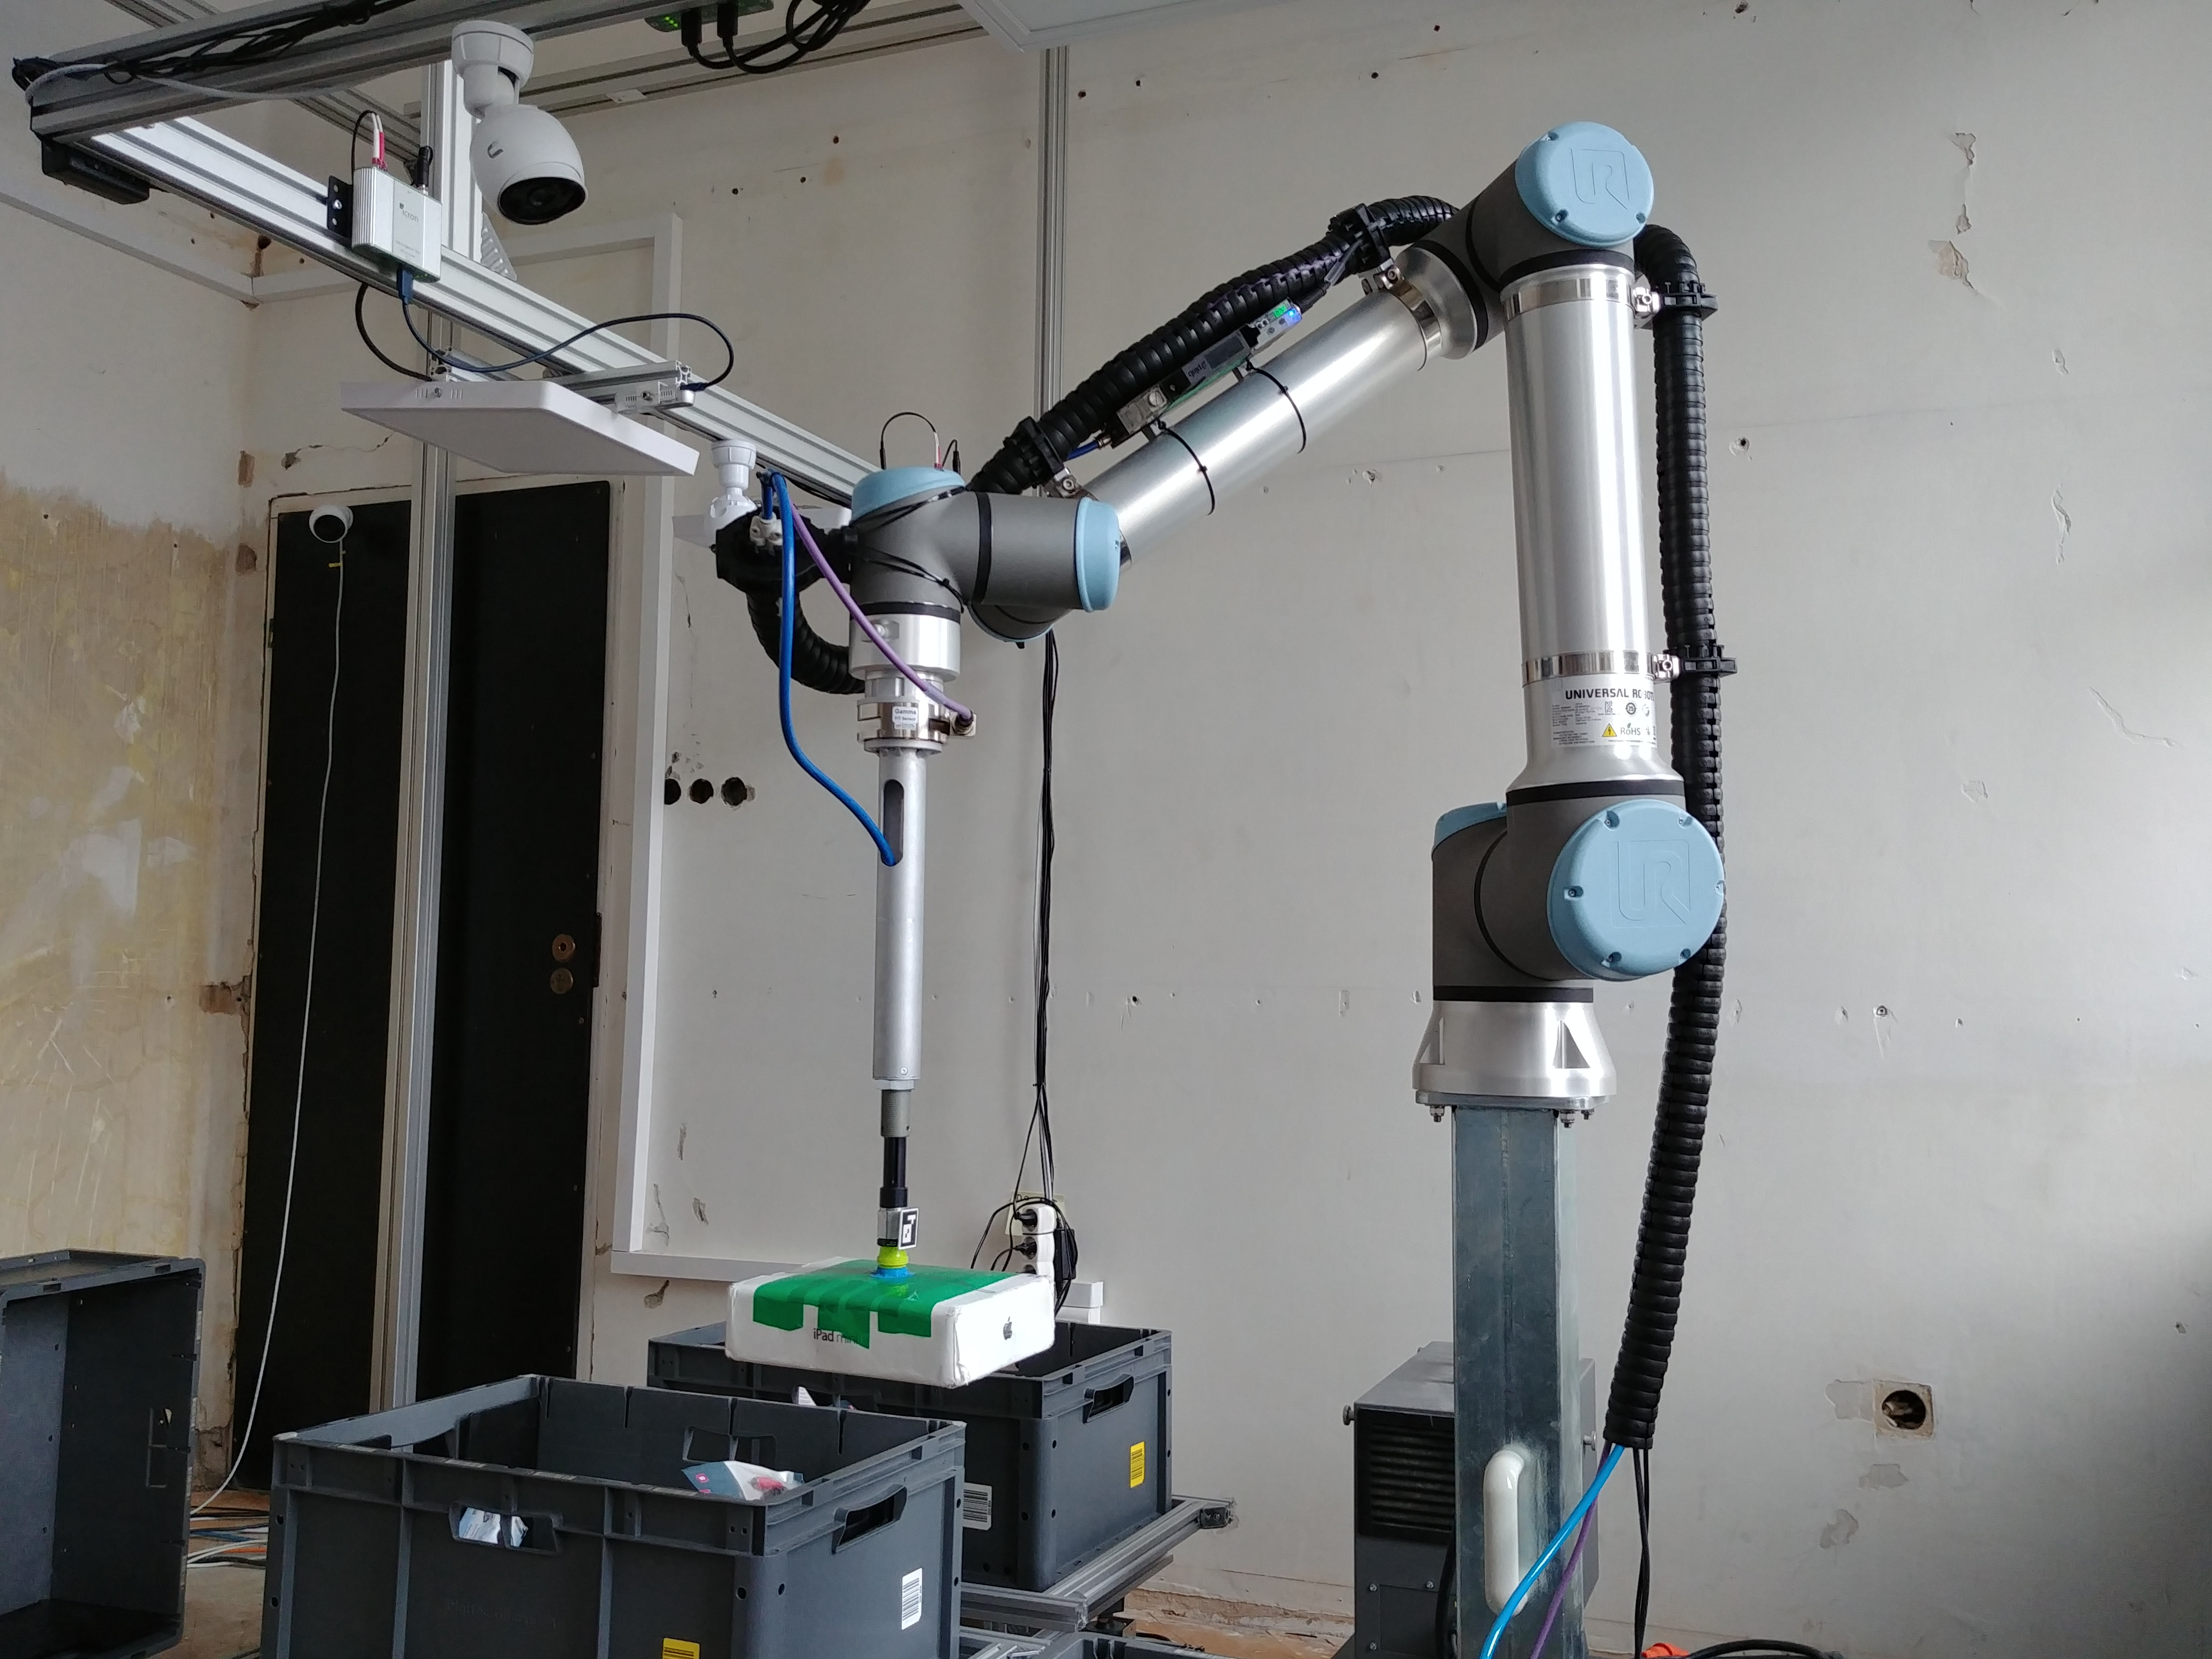
\includegraphics[scale=0.05]{\main/figures/picture_of_ur.jpg}
  \caption{Robotic arm from \textsc{Universal Robot}\texttrademark \ grasping a box. Image from the author.}
  \label{fig:background:albert}
\end{figure}

\subsection{\ac{FT} sensor}

Two \ac{FT} sensors are used within the project. The built-in sensor of UR10e and the \textit{Gamma} \ac{FT} sensor from ATI\texttrademark. They are both mounted on the last joint of both robotic manipulators (see Figure \ref{fig:background:tool}). The ATI\texttrademark \ sensor is mostly used throughout the evaluation of the different approaches. Although its range of measurement is narrower than UR10e one, it has better resolution properties (see Table \ref{table:background:ft-sensor}).

\begin{table}[h!]
  \begin{center}
    \caption{Specifications of the built-in UR10e sensor and \textit{Gamma} sensor \ref{ati, ur10e}. }
    \label{tab:background:ft-sensor}
    \renewcommand{\arraystretch}{1.8} % Default value: 1
    \begin{tabular}{l|c|c} % <-- Alignments: 1st column left, 2nd middle and 3rd right, with vertical lines in between
      & \textbf{ATI Gamma} & \textbf{UR10e}\\
      \hline
      Range (force)  & $F_{x/y}: 32 \ \si{\newton}$ $F_z: 100 \ \si{\newton}$ & \underline{$100 \ \si{\newton}$} \\
      \hline
      Range (torque)  & $2.5 \ \si{\newton} \si{\meter}$ & \underline{$10 \ \si{\newton} \si{\meter}$} \\
      \hline
      Resolution (force)  & \underline{$F_{x/y}: 0.0062 \ \si{\newton}$ $F_z: 0.012 \ \si{\newton}$} & $2.0 \ \si{\newton}$ \\
      \hline
      Resolution (torque)  & \underline{$0.0005 \ \si{\newton} \si{\meter}$} & $0.02 \ \si{\newton} \si{\meter}$ \\
      \hline
    \end{tabular}
  \end{center}
\end{table}

\subsection{End-effector}

The end-effector of the robot fullfills the functions of grasping a wide range of items, measuring the force induced on the wrist, safely picking from diverse source totes, carts or conveyors. It consists of 4 basic elements (see Figure \ref{fig:background:tool}):

\begin{itemize}
  \item an ATI\texttrademark \ sensor which is screwed on the wrist of the robotic manipulator,
  \item an extension tube to reach deep totes or carts,
  \item a second cylinder inserted in the previous one with a safety-spring,
  \item a vacuum suction cup linked to the hydraulic supply.
\end{itemize}

\begin{figure}[H]
  \centering
  \includegraphics[scale=0.05, angle=-90]{\main/figures/picture_of_tool.jpg}
  \caption{Tool mount on the robotic manipulator. Image from the author.}
  \label{fig:background:tool}
\end{figure}

A suction cup with a springy extension is mounted on the tool. It allows a very simple integration logic and a versatile ability to grasp items (see Figure \ref{fig:background:suction}). The sealing lip provide a good grip on a large range of object texture.

\begin{figure}
\centering
\begin{subfigure}{0.49\textwidth}
\centering
\includegraphics[scale=0.03]{\main/figures/suction_unloaded.jpg}
\caption{Unloaded}
\label{fig:background:suction-unloaded}
\end{subfigure}
\begin{subfigure}{0.49\textwidth}
\centering
\includegraphics[scale=0.03]{\main/figures/suction_loaded.jpg}
\caption{Loaded}
\label{fig:background:suction-loaded}
\end{subfigure}
\caption{Vaccum suction cup gripper. Images from the author.}
\label{fig:background:suction}
\end{figure}

\subsection{Characteristics of a typical \textit{pick-and-place} motion}

In the context of \textit{pick-and-place} tasks, a robotic manipulator is meant to
take an item from a given initial pose to a final pose \cite{Angeles2006}. This type of operation is exploited in tasks like loading and unloading of conveyor belts, totes, carts. In the use case of the project, trajectories have a blending trapezoidal shape. They are optimized for high production cadence and grasping failure avoidance (see Figure \ref{fig:background:tote_cycle}).

\begin{figure}[H]
  \centering
  \includegraphics[scale=0.05]{\main/figures/tote_cycle.jpg}
  \caption{Trajectory of the \ac{TCP} during a \textit{pick-and-place} cycle. Image from the author.}
  \label{fig:background:tote_cycle}
\end{figure}

The drawback of using a suction cup for grasping is that the mechanical link between the tool and the item is not rigid. Heavy items and objects with large dimension are very likely to oscillate during the motion. In logistic warehouses, robots often handles object over half a kilo and longer dimension over $0.3 \si{\meter}$. Observations show that the angle between the tool and the item may vary significantly (up to $10 \si{\degree}$). Wobbling has a knock-on effect on \ac{FT} measurement. While there should not be any oscillations of the torque in a rigid model (for more detail, please refer to Section \ref{section:mechanical-models}), significant variations can be seen in actual measurement (see Figure \ref{fig:results:torque_}).

When it comes to physically model the system, different level of details can be take into account. The first approach is to considered a rigid link between the tool and the item and a second approach is to fit an appropriate mechanical model considering the number of \ac{DoF} and the damped harmonic oscillator theory.


\section{Mechanical models}
\label{section:mechanical-models}

A lot of effort have been put into estimating the dynamic parameters of each rigid body link of robotic manipulators during the late century spent. An et al. \cite{An1985} have developped a method to estimate the mass, the location of the center of mass and the moment of inertia of every link of a robotic arm. The method uses the joint torques and the calculation of the kinematics of the manipulator while moving. This work provide a sound method to derive the dynamic equations (see Section \ref{subsubsection:background_newton_equation} and \ref{subsection:method_newton_equation}).

\textit{TODO}

\begin{figure}
  \centering
  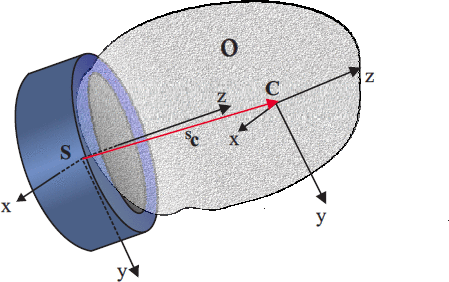
\includegraphics[scale=0.4]{\main/figures/scheme.png}
  \caption{\ac{FT} sensor with an object rigidly attached. Image from \cite{Kubus2007}}
\end{figure}

\begin{itemize}
 \item \ac{FT} sensor measuring: force $f$ and torque $\tau$,
 \item payload attached to the \ac{FT} sensor: mass $m$, center of mass $c$, moment of inertia $I$, linear acceleration $a$, angular acceleration $\alpha$, angular velocity $\omega$,
\end{itemize}

\subsection{Rigid model of the \{tool + item\} system}

\subsubsection{Formulation of the \textsc{Newton-Euler} equations}
\label{subsubsection:background_newton_equation}

\textit{TODO}

Dynamic model of the load rigidly attached to the manipulator

The motion of the body due to external forces is described by the two equations \cite{Kubus2007, Kubus2008}:

\begin{equation}
 \label{dim_1}
 \left \{
 \begin{array}{l l}
  f =    & m (a - g) + \dot{\theta} \times (\dot{\theta} \times m c) + \ddot{\theta} \times m c \\
  \tau = & m c \times (a - g)
  + I_{S} \ast \ddot{\theta} + \dot{\theta} \times (I_{S} \ast \dot{\theta})
 \end{array}
 \right.
\end{equation}

also in matrix form:

\begin{equation}
 \begin{pmatrix}
  f    \\
  \tau
 \end{pmatrix}
 = A(a, \alpha, \omega, g) \varphi
\end{equation}

with $\varphi = (m, m c_x, m c_y, m c_z, I_{xx}, I_{xy}, I_{xz}, I_{yy}, I_{yz}, I_{zz}) {}^T$

\subsection{\ac{RMSD} model of the \{tool + item\} system}


\subsection{Sensor offset}

\textit{TODO}

{\it
Strategies to manage the (unknown) sensor offset \cite{Kubus2007, Kubus2008}.
}

\section{Estimation Approaches}

\subsection{Least-Squares method}

\textit{TODO}

{\it
Brief presentation of the method in order to highlight the limit of the least-squares method.
}

\subsection{Recursive Total Least-Squares technique}

\textit{TODO}

{\it
Recursive Total Least-Squares considers error $E$ in the data matrix and error $e$ in the \ac{FT} vector \cite{Kubus2008}
.

\begin{equation}
 \begin{pmatrix}
  f    \\
  \tau
 \end{pmatrix} + e
 = (A + E) \varphi
\end{equation}
}

\end{document}
